\documentclass[titlepage,10pt]{article}
\usepackage{textcomp}
\usepackage{latexsym}
\usepackage{graphicx}
\usepackage{amsmath}
\usepackage{moreverb}
%\usepackage[hmargin=3cm,vmargin=3.5cm]{geometry}

\def\urltilda{\kern -.15em\lower .7ex\hbox{\~{}}\kern .04em}


\begin{document}
\title{
Scaled SWIFT \\
Research Proposal
}

\author{Zouhair Mahboubi}

\date{February 11$^{th}$, 2010\\ Stanford University}

\maketitle
\newpage

\abstract
This paper is meant to be a quick overview of the research potential of building a scaled SWIFT model. The goal of the research is to understand effects of scaling on the aerodynamic performance and dynamic response of sub-scale models. We hope to eventually establish a theory and framework to compensate for these effects, in order to be able to better predict in the future for which maneuvers the performance and dynamic parameters obtained from the sub-scale are representative of the full-scale. \\

In the paper, we motivate our choice of the SWIFT as a platform and highlight the potential of collaboration with NASA Ames. We then present some preliminary results of weight, power and price estimation as well as aerodynamic performance for 3 different scales (1/2, 1/3 and 1/4) 

\newpage
\section{Introduction}
The SWIFT is a foot-launched hang-glider with performance similar to a sailplane. The plane has been flown for many years and won numerous competitions. It has also been converted to a powered plane in a pusher-prop configuration. Recently, NASA Ames Research Center (ARC) purchased one of these planes and is planning on converting the airplane into an electrically powered Unmanned Aerial Vehicle (UAV) that would be capable of serving as a technology demonstrator.\\
Our goal is to develop one or two sub-scale models of the SWIFT which can be used as a platform for research in both controls and applied aerodynamics. We intend to coordinate our efforts with the on-going research on the full-scale aircraft, in the hope that data, algorithms, models, etc. can be shared and used on both vehicles.

\section{Motivation}
\subsection{the SWIFT as a platform}
Generally speaking, the weight of a scale-model is proportional to the cube of the scale. With a smaller weight and surface area, the drag of the model airplane and therefore the propulsive power requirement are significantly smaller. With the lower power requirements and reduced weight, a model plane is safer to operate, and cheaper to construct and maintain. Turn-around time for flight-tests is also quicker given the reduced complexity of flight-logistics: model aircrafts are regulated by the Academy of Model Aeronautics (AMA), whereas UAVs operating in the NAS must follow FAA guidelines and need to obtain a permit.\\

In the short term, a scale-model of the SWIFT could be used by NASA-ARC for testing planned modifications or new control algorithms before implementing them on the full-scale plane. This means the possibility of demonstrating new concepts quicker, safer and cheaper. \\

\enlargethispage{2\baselineskip}
The difficulty is in ensuring that the model will have performance and handling qualities similar to those of the full-scale. In order to do this, the scaling needs to maintain some similitude requirements \cite{Wolowicz} (non-dimensional coefficients describing the aerodynamics and dynamics need to be matched). However, it is usually difficult to have all of them matching. And although the use of scale-models for testing aircraft performance is not a new concept, it is still unclear how much error is introduced by incorrect scaling. For these reasons, the SWIFT is an attractive platform given that we would have access to flight-test data of both the model and scale airplanes, thus allowing us to quantify uncertainties on the estimates of performance and dynamic properties caused by unmatched similitude coefficients. Per example, it would be possible to find out which stability derivatives can be trusted from system identification when Reynolds numbers are not matched. We would then investigate methods to account for the discrepancies.\\

\subsection{Research Applications}
The main goal of this project is to establish a theory and framework which would lead to a better understanding of effects of scaling on aerodynamic performance and dynamic response. In the process, we plan to come-up with methods that would account for these effects in order to better predict the performance of the full-scale model.\\

But since we will have at our disposal a UAV with a relatively high aerodynamic efficiency, we can use it as a testbed for other on-going projects within the Aircraft Design Group: per example dynamic soaring, or characterization of propeller noise (and how it scales). \\

The SWIFT has a low wing loading, and is likely to benefit from solar power. But it's unclear how the addition of panels to the wing affect the airfoil's performance (changing roughness, turbulence onset, etc.) and how the solar-power can be optimally integrated with battery power. This can be investigated on the sub-scale model, and alongside the other applications, could eventually benefit NASA's full-scale UAV. 

\subsection{Literature review}
As mentioned before, the use of models for testing aircraft concepts is not new. NASA itself has a history of using unmanned sub-scale models such as the X-38 Crew Return Vehicle, or the more recent X-48 Blended-Wing-Body demonstrator. But generally speaking, the trend is to construct a scaled model to demonstrate a new technology, before the full-scale airplane is built. One can imagine that at the prototype stage, much of the design is not yet frozen and the full-scale is likely to be different from the sub-scale, thus making it hard to compare flight-test results between the model and the full-scale.\\

A notable exception is NASA's AirSTAR program in which a 5.5\% dynamically scaled version of a B757 was built. The focus of the program however is on 'Integrated Resilient Aircraft Control' which would help prevent loss-of-control accidents. As mentioned in \cite{Airstar} "AirSTAR testbed will be used for [experiments] such as loss-of-control flight due to high angles-of-attack and sideslip, [where] the flow around the aircraft becomes separated and fluid effects associated with Reynolds number scaling may be minimized. For more benign flight conditions, Reynolds number effects can be significant and the aerodynamics of the model would not be representative of the full scale aircraft for certain maneuvers."\\

Our goal is different in that we want to actually understand how significant these effects can be, in order to be able to better predict in the future for which maneuvers the performance and dynamic parameters are representative.

\section{Methodology}
\subsection{Initial Sizing}
Based on initial sizing, we believe that a 1/3 scale-model would be useful while remaining manageable. A 1/2 scale is doable with off-the-shelf RC hobbyist parts but the logistics are somewhat harder.


We plan to use traditional methods for the construction (i.e. foam-core and balsa wood mostly) and rely on off-the-shelf RC hobbyist parts and materials to keep the cost down. Initial weight and price estimates (alongside some assumptions) are summarized in Table \ref{tab:scales} and figure \ref{fig:scales}. The details of the computation steps are given as comments in the Spreadsheet.

\begin{table}[h]
\begin{center}
\begin{tabular}{|c|c|c|c|c|}
\hline
Scale $\lambda$	& 1 & 1/2 & 1/3 & 1/4 \\ \hline
Span (m)	& 13& 6.5 & 4.3 & 3.25\\ 
Mass (kg)	& 150& 17 & 5   & 3 \\
Cruise(m/s)	& 17 & 11 & 9   & 8.9 \\
$Re_{avg}$  	& 1,150,000 & 370,000 & 200,000 & 150,000 \\
Froude		& 29.5 & 24.5 & 25.3 & 32.3 \\
Power (W)	& 6520 & 527 & 130 & 70 \\
Price (\$)      & $>$40000 & 4500 & 2500 & 2000 \\
\hline
\end{tabular}
\caption{Scale Comparison}
\label{tab:scales}
\end{center}
\end{table}


The price estimates for the models are for the material and components and include about \$1000 for the autopilot and sensors \footnote{This is likely under-estimated, especially if we want high-accuracy sensors/}. It should be noted that the 1/2 scale values might be inaccurate since the construction method is likely to be different, nonetheless, they should be rough estimates. Figure \ref{fig:scales} plots the ratios of these estimates relative to the full-scale airplane. These results which are obtained from individual component build-up seem to agree with the 'rule of thumb' that mass is roughly cubic in the scale $\lambda$. Price and power are strongly dependent on weight so it's no surprise that their trends are similar to the mass. We also notice that the Reynolds number varies with $\lambda^{1.5}$: this is expected since if the mass is cubic in scale and lift-coefficient is assumed to be constant, the velocity varies with $\sqrt{\lambda}$. The Froude number $Fr =\frac{V^2}{g \bar{c}}$ so it should be proportional to $\frac{{\sqrt{\lambda}}^2}{\lambda}=1$, which explains why the ratio is 'around' 1.

\begin{figure}[h]
\begin{center}
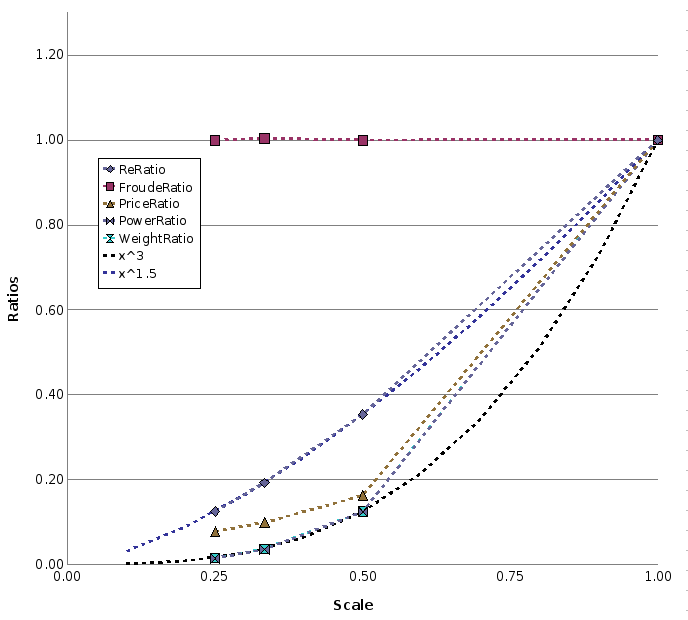
\includegraphics[width=140mm]{scale-graph.PNG}
\end{center}
\caption{Similitude Parameters versus Scale}
\label{fig:scales}
\end{figure}

\clearpage

\subsection{Autopilot and Sensors}
We are likely to fly the airplane with a remote controlled radio before moving to an automous vehicle. But even in the initial phases, having an autopilot which serves as an 'avionics' unit to log inputs and responses of the aircraft.\\

Since our goal is not particularly to develop a new autopilot, an off-the-shelf one would be preferable. We require a board that has enough PPM channels to command at least 8 servos and one Electronic-Speed-Controller, 3 serial ports (radio, GPS and IMU) and 5 to 8 A2D converters for the alpha-beta veins, pressure sensors, etc. Unfortunately, most commercially available autopilots are closed-source and tend to be cost-prohibitive, which forces us to turn to the DIY scene. However, even the most mature DIY systems have limited processing power, serial and I/O ports.\\

For these reasons, we are considering to use the open-source \textit{Paparazzi} software in conjunction with a \textit{Roboard} hardware. We chose this architecture because the \textit{Roboard} hardware satisfies our requirements. This is approach has been done by other people, and the paparazzi has a good track record of habing being used on different hardware architectures (ranging from Gumstix to x86 computers). The point is that we could develop our own autopilot from scratch, but the hope is to avoid 'yet-another-autopilot' by leveraging the \textit{Roboard} and \textit{Paparazzi} capabilities since they are both open source. 

\subsection{Issues with small Reynolds numbers}
A 1/4 scale has the advantage of being roughly the size of most RC models, which means that flying it would be relatively easy. The problem however, is that at this scale Reynold numbers are so small that the airfoil characteristics are likely to suffer, especially at high lift-coefficients. In order to analyze the effect of this, we have used Xfoil to generate section data at different Reynolds numbers. We then used the results with a vortex-lattice code (XFLR5, \ref{fig:xflr3D} is a sample view of the 3D geometry) to generate angle-of-attack sweeps for the different scales and masses. The lift was constrained to match the weight so that different velocities and Reynolds numbers are used. The curves are truncated after one of the wing's sections stalls since the data can no longer be interpolated. \\

\begin{figure}[h]
\begin{center}
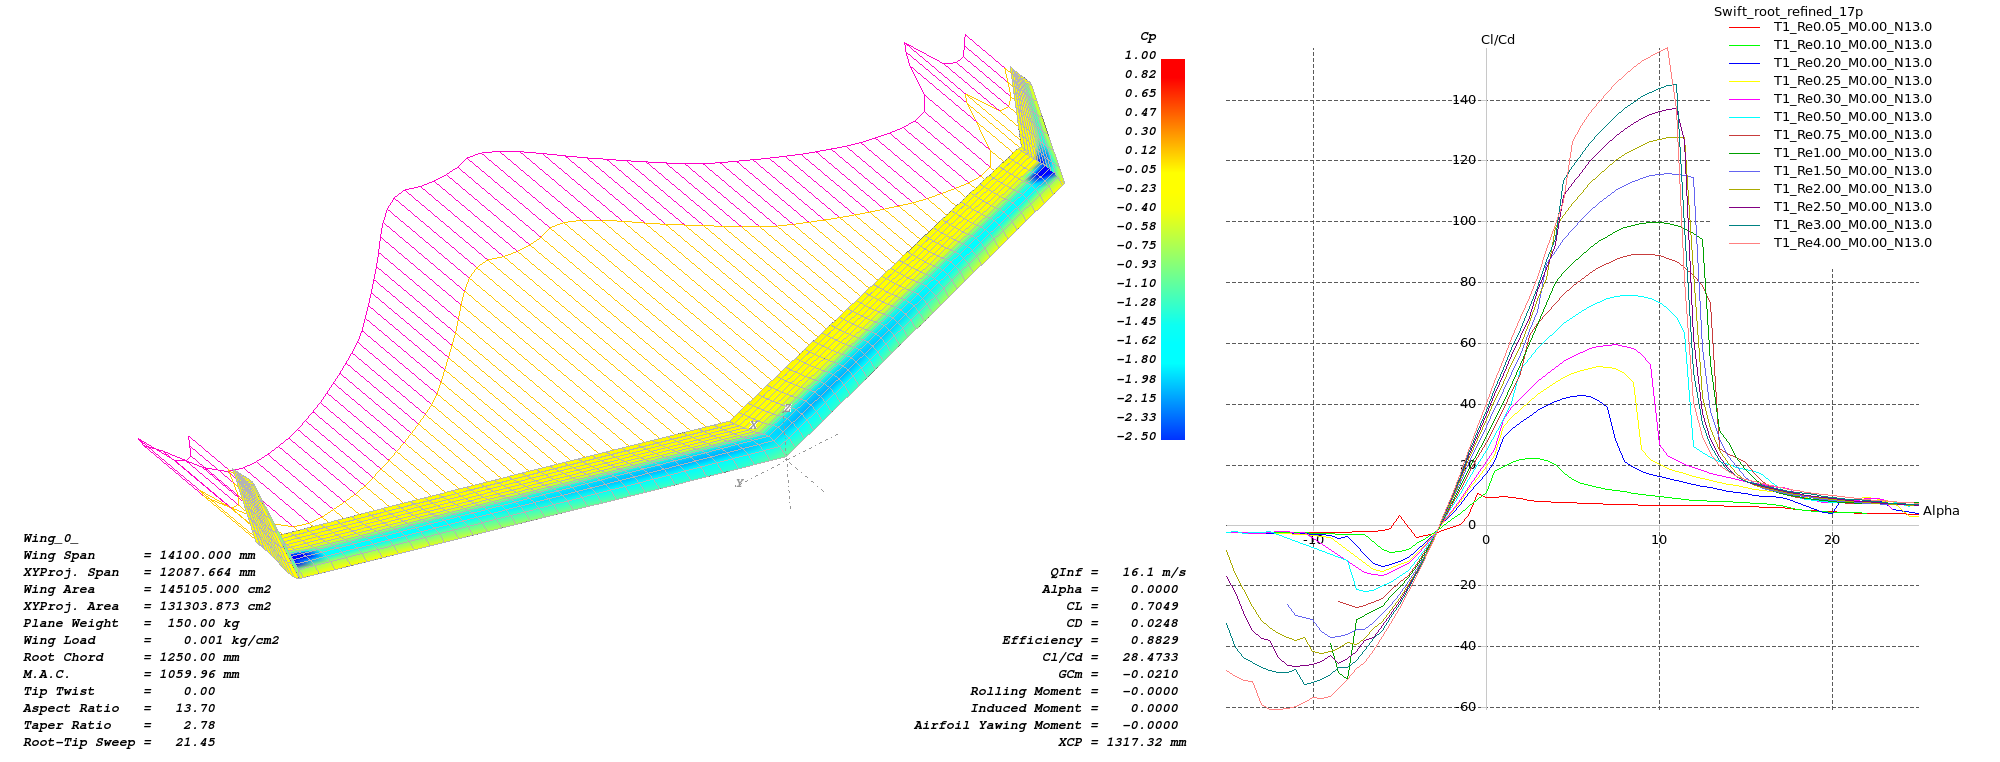
\includegraphics[width=120mm]{XFLR_3Dviews.png}
\end{center}
\caption{3D Geometry and $\frac{CL}{CD}$ for typical section at different Re numbers}
\label{fig:xflr3D}
\end{figure}
\newpage
The results \footnote{The wing is at an incidence of $10^o$, Flap deflections not taken into account} of using the same 18\% thick sections at different scales are shown in figure \ref{fig:tc18}. We notice that while the full-scale achieves a maximum CL of 1.2, the 1/3 scale has $CL_{max}=0.6$ and the 1/4 scale barely reaches $CL_{max}=0.5$. Considering that we expect to cruise at $CL=0.7$, this is clearly unacceptable.

\begin{figure}[h]
\begin{center}
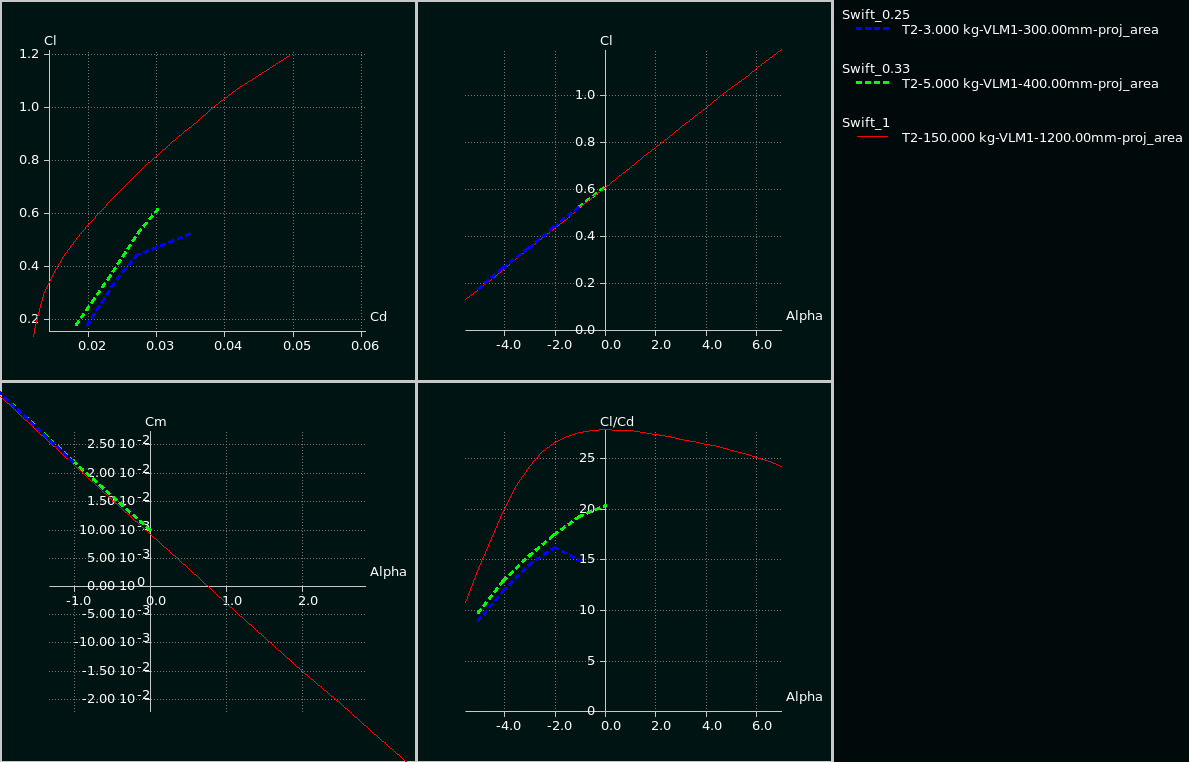
\includegraphics[width=120mm]{scale_original_airfoil.png}
\end{center}
\caption{18\% thick Airfoil for all scales}
\label{fig:tc18}
\end{figure}

\enlargethispage{6\baselineskip}
In order to fix this, we have decided to reduce the thickness to chord ratio of the airfoil sections while retaining the same camber line. This helps the flow to remain attached at higher lift coefficients despite the reduced Reynolds number. We considered both 14\% and 10\% sections, and the results are shown in figures \ref{fig:tc14} and \ref{fig:tc10} respectively. The 14\% sections would allow the 1/3 scale model to achieve $CL_{max}=0.9$ and $CL_{max}=0.8$ for the 1/4. In both cases, the pitching moment coefficient \footnote{CG position relative to the leading edge is at the same fraction of the MAC for all scales} is only slightly changed. On the other hand, the 10\% sections would allow both the 1/3 and 1/4 scale to achieve $CL_{max}=1$, but at the cost of changing the pitching moment coefficient. However, the predicted $Cm_{\alpha}$ seems to remain unchanged, so this might be acceptable since we can always move the CG position further forward to trim the models. It's worth pointing out that the drag coefficient for the scale models is higher \begin{footnotesize}(Airfoils have generally lower L/D at lower Re. Moreover, the flow on the lower surface is forced to transition at 50\% while it's not for higher ones -in both cases xtran=25\% on the top- This helps the flow remain attached at small AoA, which is important for the washed-out tip sections.)\end{footnotesize}\\
Based on this analysis, a 14\% thick section for the 1/3 model and a 10\% thick section for the 1/4 model would mitigate the low Reynolds numbers issues for most of the flight envelope.


\begin{figure}[h]
\begin{center}
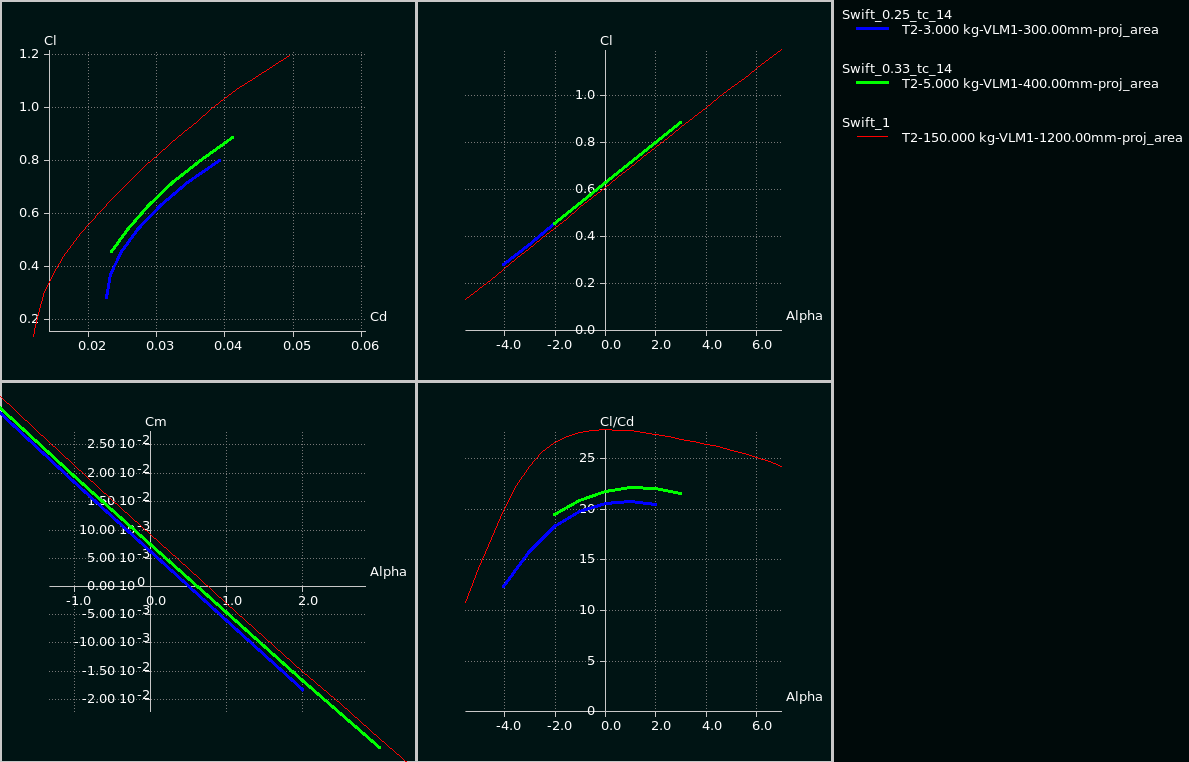
\includegraphics[width=120mm]{scale_tc_14.png}
\end{center}
\caption{14\% thick Airfoil for 1/4 and 1/3 scales}
\label{fig:tc14}
\end{figure}

\begin{figure}[h]
\begin{center}
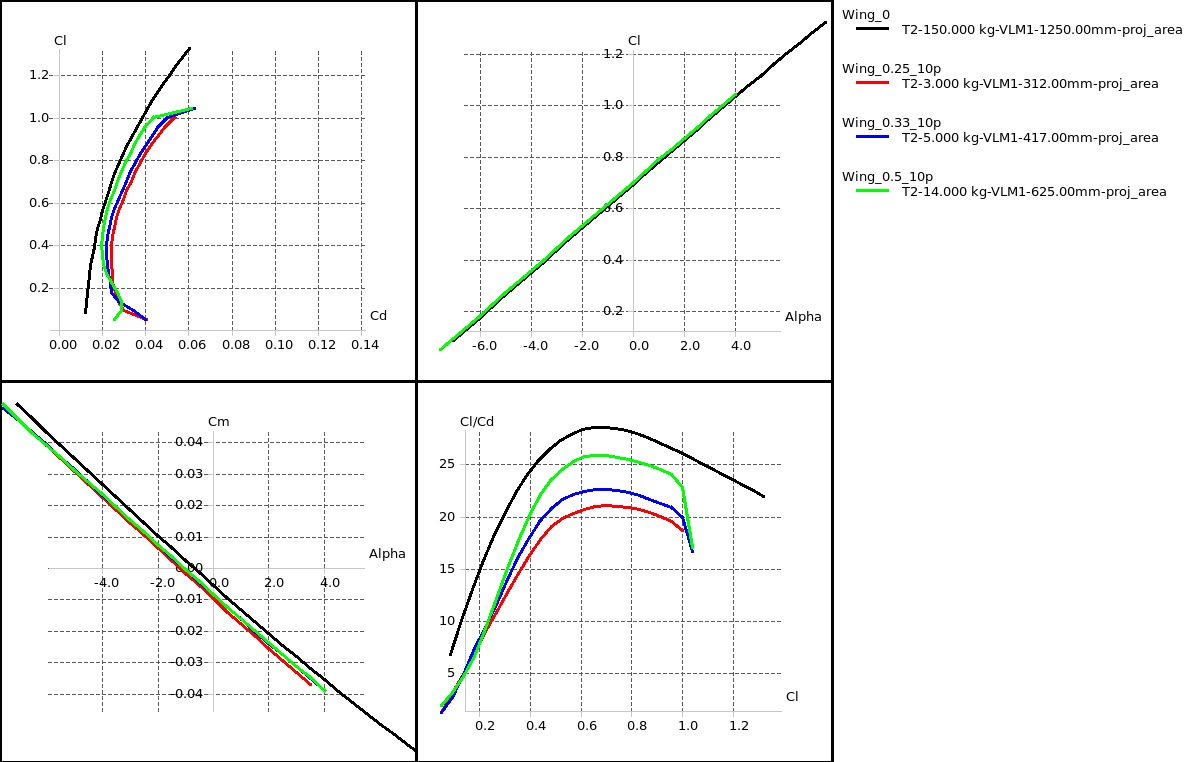
\includegraphics[width=120mm]{scale_tc_10.png}
\end{center}
\caption{10\% thick Airfoil for 1/4 and 1/3 scales}
\label{fig:tc10}
\end{figure}

\clearpage

\subsection{Inertia Measurements}
In order to estimate the aerodynamic coefficients from flight-tests, it is usually necessary to have good estimates of the mass and inertia properties of the airplane. While it is relatively easy to measure inertias for the sub-scale aircraft through a series of single degree-of-freedom oscillations, it can be a more challenging task for a full-scale aircraft where it's unsafe to hang the plane in all degrees, and therefore a meticulous component build-up is required.  We believe that it might be possible to estimate moments of inertia from flight-tests as well. The idea would be to carry-out different flights where the weight and mass distribution of the airplane are carefully changed. Because the aerodynamic performance would remain unchanged (stability derivatives are only a function of the planform), it would be possible to estimate the inertia properties more accurately. We plan to investigate this technique on the small-scale plane and hopefully apply it to the full-scale one.\\

\subsection{Time-line}
This is a very rough time-line... \\
Design in January 2010 \\
Construction of 1/4 scale in February 2010 \\
Test-flying 1/4 scale in March-April 2010 \\
Construction of 1/3 scale May-June 2010 ?\\
Test-flying 1/3 scale over summer ?? \\


\begin{thebibliography}{9}

\bibitem{Wolowicz}
   Wolowicz, C.H., Bowman, Jr., J.S., and Gilbert, W.P.,
   “Similitude Requirements and Scaling Relationships as Applied to Model Testing”, 
   NASA TP-1435, 1979.

\bibitem{Airstar}
Thomas L. Jordan, et Al.,
"AirSTAR: A UAV Platform for Flight Dynamics and Control System Testing"
NASA Langley Research Center, Hampton, VA 23681




\end{thebibliography}


\end{document}
